\chapter{Steganografie}
Die Steganografie bezeichnet eine weitere Methode die Vertraulichkeit eines
Nachrichtenaustausches zu gewährleisten.
Es wird das Ziel verfolgt, eine Nachricht in einer für den Computer
zugänglichen Trägerdatei (engl. \textit{cover media}) zu verstecken, sodass eine
weitere Person die Existenz
einer geheimen Botschaft gar nicht erst vermuten würde. Eine Trägerdatei, unempfindlich
gegenüber kleinen Änderungen in den Daten eignet sich besonders gut für die
Anwendung steganografischer Verfahren. Digitale Bilddateien sowie Audio- und Videodateien
sind sehr geeignete Trägermedien,
da ihre Daten ein ganz natürliches Rauschen aufweisen.
In diesem Kapital soll ein Algorithmus vorgestellt werden, welcher
eine beliebig lange Nachricht in einem Bild versteckt und versucht,
die visuelle Qualität des Urbilds zu bewahren.

\section{Modifikation von Bilddateien}
Eine digitale Bilddatei besteht aus einer zweidimensionalen Anordnung von Pixel, wobei
jeder eine bestimmte Farbe annehmen kann. Farben können unterschiedlich
dargestellt werden, dass in der Bildwiedergabe am häufigsten verwendete Modell ist
der RGB-Farbraum. Die Farbwahrnehmung des menschlichen Auges kann durch
das additive Mischen der drei Grundfarben Rot, Grün und Blau (RGB)
nachgebildet werden \parencite[32-40]{BOOK:VC}. In computerorientierten Anwendungen
werden hierfür pro Farbkanal Zahlenwerte zwischen 0 und 255 gespeichert,
es gilt je größer der Wert desto heller die Farbe. Die Kombinationen
$(255,0,0)$, $(0,255,0)$ und $(0,0,255)$ beschreiben jeweils die Grundfarben Rot, Grün und Blau.
Das Mischen aller Farben $(255,255,255)$ ergibt Weiß und das Hinzufügen gar keines
Lichts $(0,0,0)$ resultiert in Schwarz. Kombinationen mit gleicher Intensität
$(100,100,100)$ werden als Grauton wahrgenommen. Pro Pixel müssen in einem Bild
also drei Byte an Information gespeichert werden, dies verspricht ein großes
Potenzial, wenn es darum geht, unentdeckt Information zu verbergen. Ein
einfaches und effektives Verfahren ist das Überschreiben der niederwertigsten
Bit im Farbkanal durch das zu versteckende Signal. Das Anpassen
der niederen Stellenwerte verändert den Farbwert nur minimal und
die kleinen Abweichungen werden nur durch betrachten des veränderten Bilds
nicht zu erkennen sein.

\paragraph{Wie stark kann ein Bild angepasst werden?}
Es soll nun abgeschätzt werden, wie stark eine gegebenes Bild verändert
werden kann, ohne dass die Qualität des Resultats sichtbar beeinflusst
wird. Es seien $b_7\,b_6\, \ldots \,b_0$ die acht Bit eines Farbkanals, es soll für
jeden Kanal der maximale Fehler betrachtet werden, welcher entstehen kann,
wenn die $n$ niederwertigsten Bit durch eine Nachricht ersetzt werden.
Der neue Farbwert inklusiv Fehler wird nach \eqref{eq:bit-max-error} in Bezug auf $n$ bestimmt:

\begin{equation}
  a(n) = \sum_{i=0}^{n - 1} b_i \cdot 2^i \qquad
  b_{i, n} =
  \begin{cases}
    b_i & \text{wenn $i \geq n$}                                                           \\
    1   & \text{wenn $a(n) \leq \lfloor \frac{1}{2} \cdot \sum_{i=0}^{n - 1} 2^i$} \rfloor \\
    0   & \text{sonst}
  \end{cases}
  \label{eq:bit-max-error}
\end{equation}

\begin{example}
  Es werden die letzten vier Bit betrachtet ($n = 4$):
  \begin{align*}
    b_7\,b_6\, \ldots \, b_0 & = 10010110 & b_{7,4}\,b_{6,4}\, \ldots \, b_{0,4} & = 10011111 \\
    b_7\,b_6\, \ldots \, b_0 & = 10011110 & b_{7,4}\,b_{6,4}\, \ldots \, b_{0,4} & = 10010000
  \end{align*}
\end{example}

\noindent
Die Auswirkungen des Fehlers auf ein Bild für alle möglichen $n$
sind in \autoref{fig:peppers} zu sehen. Es kann die durchaus vielversprechende Beobachtung
gemacht werden, dass Änderungen bis hin zur vierten Stelle im Farbkanal nur schwer und
ohne Vergleich mit der Originaldatei wahrscheinlich nicht erkannt werden würden.
Zusätzlich wurde in diesem Beispiel der schlimmste Fall betrachtet und das Verstecken
einer echten Nachricht wird fast immer ein besseres Ergebnis liefern, da die Bit der Nachricht
zufällig mit den des Bilds übereinstimmen.

\begin{figure}[t!]
  \centering
  \begin{minipage}[t]{0.3\textwidth}
    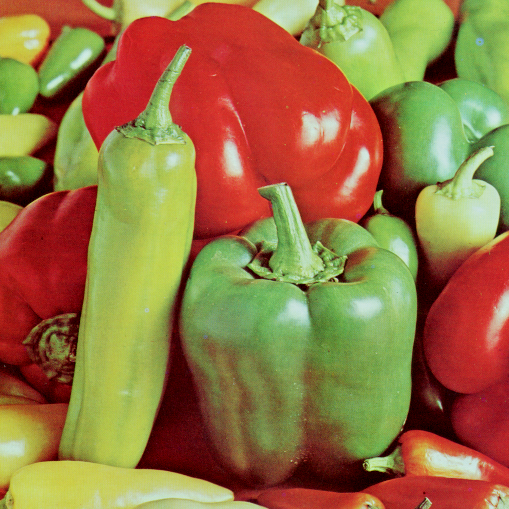
\includegraphics[width=1\textwidth]{peppers-0.png}
    \caption*{$n = 0$ (Original)}
  \end{minipage}
  \hfill
  \begin{minipage}[t]{0.3\textwidth}
    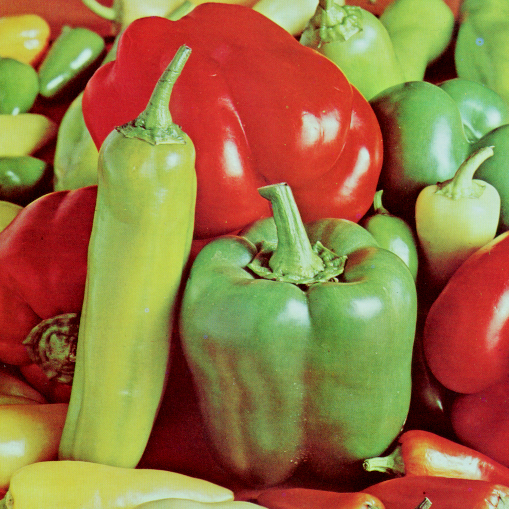
\includegraphics[width=1\textwidth]{peppers-1.png}
    \caption*{$n = 1$}
  \end{minipage}
  \hfill
  \begin{minipage}[t]{0.3\textwidth}
    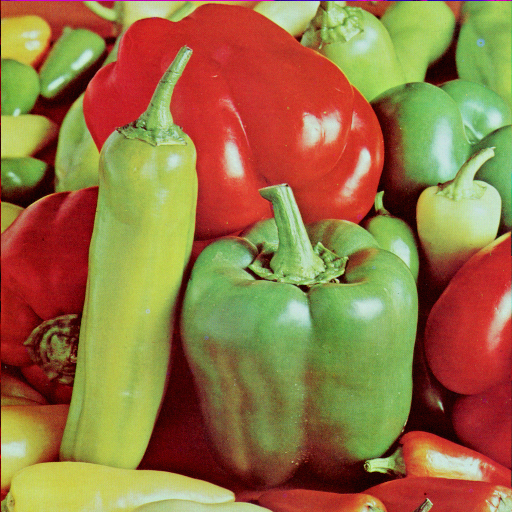
\includegraphics[width=1\textwidth]{peppers-2.png}
    \caption*{$n = 2$}
  \end{minipage}%
  \vspace{0.5cm}
  \begin{minipage}[t]{0.3\textwidth}
    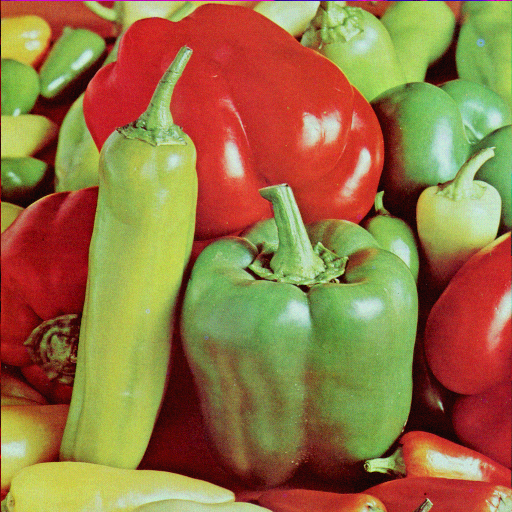
\includegraphics[width=1\textwidth]{peppers-3.png}
    \caption*{$n = 3$}
  \end{minipage}
  \hfill
  \begin{minipage}[t]{0.3\textwidth}
    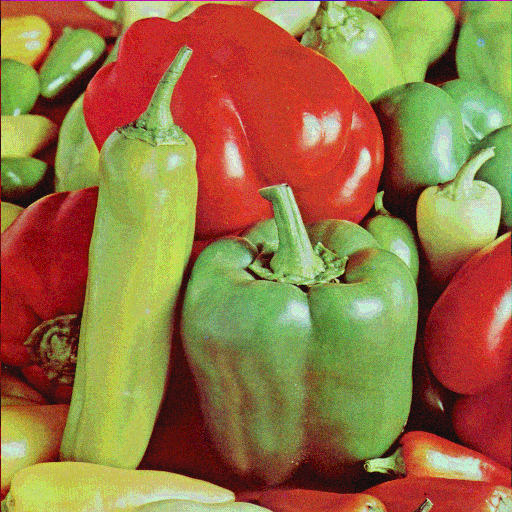
\includegraphics[width=1\textwidth]{peppers-4.png}
    \caption*{$n = 4$}
  \end{minipage}
  \hfill
  \begin{minipage}[t]{0.3\textwidth}
    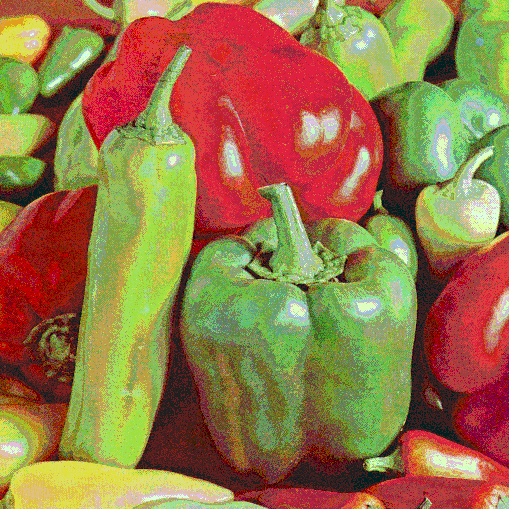
\includegraphics[width=1\textwidth]{peppers-5.png}
    \caption*{$n = 5$}
  \end{minipage}%
  \vspace{0.5cm}
  \begin{minipage}[t]{0.3\textwidth}
    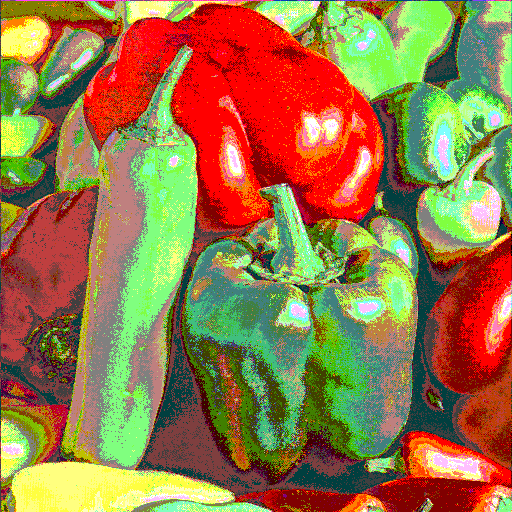
\includegraphics[width=1\textwidth]{peppers-6.png}
    \caption*{$n = 6$}
  \end{minipage}
  \hfill
  \begin{minipage}[t]{0.3\textwidth}
    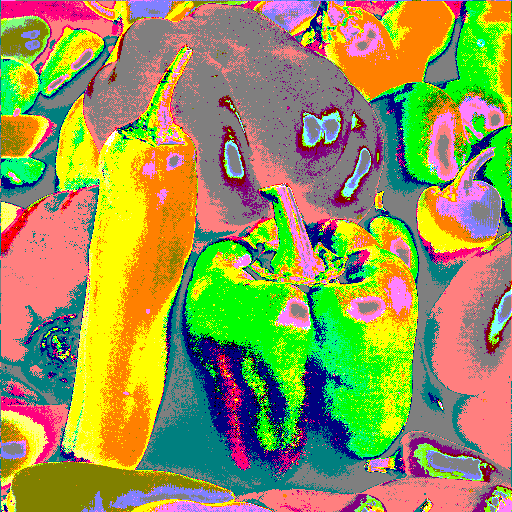
\includegraphics[width=1\textwidth]{peppers-7.png}
    \caption*{$n = 7$}
  \end{minipage}
  \hfill
  \begin{minipage}[t]{0.3\textwidth}
    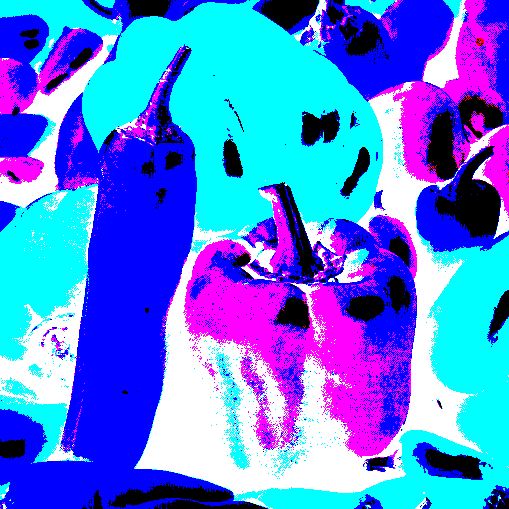
\includegraphics[width=1\textwidth]{peppers-8.png}
    \caption*{$n = 8$}
  \end{minipage}
  \caption{Farbbild Paprika veränderten durch maximalen Fehler für alle $n \in [0,8]$.}
  \label{fig:peppers}
\end{figure}


\section{Algorithmus}

\begin{figure}
  \centering
  \begin{minipage}[t]{0.45\textwidth}
    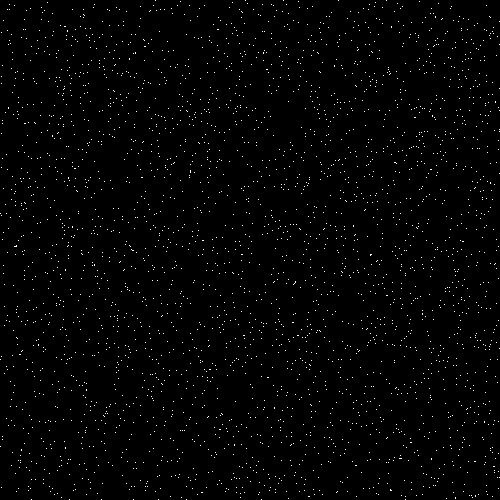
\includegraphics[width=1\textwidth]{black-1200.png}
    \caption*{1200 Byte}
  \end{minipage}
  \hfill
  \begin{minipage}[t]{0.45\textwidth}
    
\includegraphics[width=1\textwidth]{black-3600.png}
    \caption*{3600 Byte}
  \end{minipage}%
  \vspace{0.5cm}
  \begin{minipage}[t]{0.45\textwidth}
    
\includegraphics[width=1\textwidth]{black-10800.png}
    \caption*{10800 Byte}
  \end{minipage}
  \hfill
  \begin{minipage}[t]{0.45\textwidth}
    
\includegraphics[width=1\textwidth]{black-32400.png}
    \caption*{32400 Byte}
  \end{minipage}
\end{figure}